\documentclass{beamer}
\usepackage{beamerthemeshadow}
\usepackage[spanish]{babel}
\usepackage[utf8]{inputenc}
\usepackage{multicol}

\mode<presentation> {
  \setbeamercovered{transparent}
}

% Code for placing the footnote above the navigiation symbols
\addtobeamertemplate{footnote}{\vspace{-6pt}}{\vspace{6pt}}
\makeatletter
\setbeamerfont{footline}{size=\fontsize{4}{6}\selectfont}
\setbeamerfont{headline}{size=\fontsize{4}{6}\selectfont}
% Alternative A: footnote rule
\renewcommand*{\footnoterule}{\kern -3pt \hrule \@width 2in \kern 8.6pt}
% Alternative B: no footnote rule
% \renewcommand*{\footnoterule}{\kern 6pt}
\makeatother

\begin{document}
\title{Workshop de Git}  
\author{Iván Badgen, Pablo Rago}
\institute{Despegar.com}
\date{\today} 

\begin{frame}
\titlepage
\end{frame}

\begin{frame}{Contenido}
\begin{multicols}{2}
\tableofcontents
\end{multicols}
\end{frame}

\section{Introducción} 

\begin{frame}\frametitle{¿Qué es Git?} 
  \begin{block}{Definición}
    Git es un sistema de control de versión libre, de código abierto y \textbf{distribuido}, diseñado
    para manejar desde proyectos chicos a muy grandes en forma veloz y eficiente. \footnotemark
  \end{block} \pause
  
  \begin{block}{Comentario}
    Así como se denomina distribuido, en realidad nosotros lo usamos en forma centralizada. Cuando mandamos nuestros cambios,
    lo hacemos a un repositorio remoto. De todos modos, cada uno tiene en su máquina un repositorio con toda la información
    histórica de las ramas en las que trabajamos, aún cuando no tenemos conexión al servidor, y se puede configurar para usarlo en forma
    distribuida. 
  \end{block}
  \footnotetext{\url{http://git-scm.com/}}
\end{frame}

\section{Instalación}
\subsection{Instalación}
\begin{frame}[fragile]{Instalando...} 
  \begin{block}{}
      \begin{itemize}
      \item Ubuntu (Linux): \$ sudo apt-get install git \pause
	\item	 Windows: \begin{itemize}
			\item Página oficial: \url{http://git-scm.com/download/win} 
			\item Link alternativo: \url{http://code.google.com/p/msysgit/downloads/list?can=3}
			\item Tortoise Git: \url{http://code.google.com/p/tortoisegit/}
			\item \textbf{Importante:} al instalar, poner la opción putty y no openSSH.
		      \end{itemize} \pause
      \item Mac: \url{http://git-scm.com/download/mac} \pause
      \item GUI para Eclipse: EGit (buscarlo en el marketplace)
      \end{itemize}
  
    Sea cual sea la versión, siempre disponemos de un shell donde ejecutar comandos. En linux y mac es la consola unix,
    y en windows nos instala el Git Shell. 
  \end{block}
  
\end{frame}

\begin{frame}[fragile]{Instalando... (2)}
  \begin{block}{Ayuda!}
    \begin{verbatim}
$ git --help
$ git help <comando>
     \end{verbatim}
  \end{block} \pause
  \begin{block}{En SS.OO. Unix (manual más completo que el help)}
    \begin{verbatim}
$ man git
     \end{verbatim}
  \end{block} \pause
  \begin{block}{En general (man en la web)}
    \url{http://git-scm.com/docs}
  \end{block}
\end{frame}


\subsection{Configuración}
\begin{frame}[fragile]{Configurando...}
  Ejecutamos lo siguiente en el shell de git para configurar nuestro usuario \footnote{Para más información: \url{http://wiki.despegar.it/index.php/Git}}:
  
  \begin{block}{Comandos}
  \begin{verbatim}
$ git config --global user.name "Juan Perez"
$ git config --global user.email "jperez@despegar.com"
  \end{verbatim}
  \end{block}

  Esta información va a servir para indicarle al repositorio quiénes somos y cómo mostrar nuestros commits.
  
\end{frame}

\begin{frame}\frametitle{Configurando... (2)}
  \begin{block}{Generación de claves (Unix)}
  \begin{itemize}
    \item \$ mkdir -p  $\sim$/.ssh/ \pause 
    \item \$ cd $\sim$/.ssh/ \pause 
    \item \$ ssh-keygen -C jperez@despegar.com -f id\_desp\_rsa \pause 
    \item Ir a \url{http://gitorious.despegar.it/~tu\_usuario/keys} y pegar la clave generada en id\_desp\_rsa.pub
  \end{itemize}
  \end{block}
  
\end{frame}

\begin{frame}\frametitle{Configurando... (3)}

 \begin{block}{Generación de claves (Windows)}
  \begin{enumerate}
   \item Usando putty key generator generar una clave. Bajar el binario e instalarlo. \pause 
    \item Reemplazar en Key comment el tu\_usuario@despegar.com. \pause 
    \item Guardar las constraseñas generadas. (tanto la pública como la privada) \pause 
    \item Copiar la clave que se generó (Public key for pasting into OpenSHH...). \pause 
    \item Ir a \url{http://gitorious.despegar.it/~tu\_usuario/keys} y pegar la clave generada con putty key generator.
  \end{enumerate}

  \end{block}
\end{frame}

\section{Uso de Git}

\subsection{Flujo de Git}

\begin{frame}\frametitle{Flujo de Git}
  \begin{figure}
    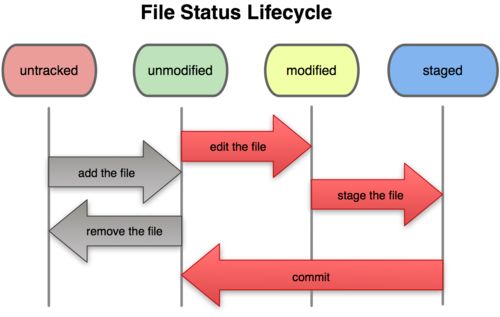
\includegraphics[scale=1]{flujo-git.png} 
    \caption{Ciclo de vida de un archivo}
  \end{figure}
\end{frame}

\begin{frame}\frametitle{Flujo de Git (2)}
  
  \begin{block}{Referencia}
    \begin{itemize}
    \item \alert{Untracked:} Archivos nuevos (similar a SVN). \pause
    \item \alert{Unmodified:} Archivos sin cambiar desde el estado HEAD de nuestro repositorio local. \pause
    \item \alert{Modified:} Archivos modificados, aún sin stage. \pause
    \item \alert{Staged:} Archivos listos para ser commiteados.
    \end{itemize}
  \end{block}
  
\end{frame}

\begin{frame}{Non-fast-forward updates}
  \begin{block}{¿Repositorio local? }
    Algo para resaltar es que, a diferencia de p. ej. SVN, lo que nosotros mandamos (\textbf{push}) al servidor no son sólo cambios, sino
    el estado completo del repositorio. Es por eso que si intentamos subir nuestros cambios mientras que otro modificó archivos,
    por más de que sean diferentes, el servidor lo va a rechazar. Nos avisa que estaríamos perdiendo cambios y nos obliga
    a hacer un \textbf{pull} para que los mezcle. Esto se conoce como non-fast-forward updates.
  \end{block}
\end{frame}

\subsection{Tiremos unos comandos}

\begin{frame}[fragile]{Comandos}
  \begin{block}{Inicializar repositorio}
    \begin{verbatim}
  $ git init
  $ git remote add origin <remoto>
  $ git add .
  $ git commit -m "Estado inicial"
    \end{verbatim}
  \end{block} \pause
  
  \begin{block}{Clonar repositorio remoto (configura automáticamente el orígen)}
    \begin{verbatim}
  # ssh (para poder hacer push)
  $ git clone git@gitorious.despegar.it:ejemplo.git
  # git (read-only)
  $ git clone git://gitorious.despegar.it:ejemplo.git
    \end{verbatim}
  \end{block}
  
\end{frame}

\begin{frame}[fragile]{Comandos (2)}
  \begin{block}{Crear ramas}
    \begin{verbatim}
  $ git branch <nombre> 
    #Crear la rama en el punto actual.                 
    # Es necesario hacer checkout a la misma.
  $ git branch <nombre> <COMMIT>    
    # Crea la rama a partir del commit dado. 
    # Es necesario hacer checkout.
  $ git checkout -b <nombre>  
    # Crear rama en el punto actual y hacerle checkout.
  $ git checkout -b <nombre> <COMMIT>   
    # Crear la rama a partir del commit dado 
    # y hacerle checkout.
  $ git branch -m <actual> <nuevo>  
    # Renombrar la rama.
    \end{verbatim}
  \end{block}
\end{frame}

\begin{frame}[fragile]{Comandos (3)}
  \begin{block}{Moverse a una rama o a un commit específico}
    \begin{verbatim}
  $ git checkout <RAMA|COMMIT>
    # No toca los cambios locales
  $ git checkout -f <RAMA|COMMIT>
    # Sobreescribe los cambios locales
    \end{verbatim}
  \end{block} \pause
  
  \begin{block}{Merge de ramas}
    \begin{verbatim}
  $ git merge <RAMA>
    # Fusiona la rama indicada en la rama actual
    \end{verbatim}    
    Las diferencias se resuelven automáticamente si es posible. En caso de conflictos,
    el proceso se detiene (merging) a la espera de una resolución manual.
  \end{block}
\end{frame}

\subsection{Conflictos... conflictos everywhere}

\begin{frame}[fragile]{Conflictos... conflictos everywhere}

  \begin{block}{Resolver conflictos por consola}
    \begin{verbatim}
$ git status                       
  # Muestra la situación actual del merge
$ git diff                         
  # Muestra los conflictos y las diferencias
$ git add <file>                   
  # Marca el archivo como mergeado
$ git rm <file>                    
  # Marca el archivo como eliminado 
  #  en la revisión definitiva
    \end{verbatim}

  \end{block}
  \begin{figure}
    
\includegraphics[scale=0.15]{everywhere.jpg} 
  \end{figure}
\end{frame}

\begin{frame}[fragile]{Conflictos (2)}

  \begin{block}{Tomar o dejar cambios}
    \begin{verbatim}
$ git checkout --ours -- <file> # Tomar el mío
$ git checkout --theirs -- <file> # Tomar el remoto
$ git reset --hard HEAD            
  # Abortar el proceso y volver a la anterior
$ git reset --hard ORIG_HEAD       
  # Deshacer si ya se había confirmado con git commit
    \end{verbatim}

  \end{block} \pause
  
  \begin{block}{Confirmando}
   \begin{verbatim}
# Confirmamos
$ git commit
$ git push <REMOTE> <RAMA>
   \end{verbatim}
  \end{block}

\end{frame}

\subsection{Conflictos con mergetool}

\begin{frame}[fragile]{Merge tool}

  \begin{block}{Configuración}
      \begin{verbatim}
  $ vim ~/.gitconfig
	
[merge]
  tool = diffmerge
[mergetool "diffmerge"]
  cmd = diffmerge --merge --result=$MERGED \ 
    $BASE $LOCAL $REMOTE
  trustExitCode = false
[diff]
  tool = diffmerge
[difftool "diffmerge"]
  cmd = diffmerge $LOCAL $REMOTE
      \end{verbatim}
  \end{block}

\end{frame}

\begin{frame}[fragile]{Merge tool (2)}

  \begin{block}{Ejecución}
      \begin{verbatim}
  $ git mergetool
      \end{verbatim}
  \end{block} \pause

  \begin{block}{Herramientas}
    Algunas opciones:
      \begin{itemize}
       \item diffmerge \pause
       \item Meld \pause
       \item Beyond Compare \pause
       \item etc...
      \end{itemize}

  \end{block}
  
\end{frame}

\section{Branching}

\subsection{Uso de Branches}

\begin{frame}[fragile]\frametitle{Creando y obteniéndose ramas}

    \begin{block}{Sujeto ``A`` empieza una feature}
      Cuando creamos una rama, se desprende de aquella en la que estamos parados. (\$ git status)
      \begin{verbatim}
$ git checkout -b feature-nueva
$ git push origin feature-nueva
      \end{verbatim}
    \end{block} \pause
    
    \begin{block}{Sujeto ''B'' quiere trabajar en la misma feature}
      \begin{verbatim}
$ git fetch origin
$ git branch -a
# *master
# remotes/origin/HEAD -> origin/master
# remotes/origin/feature-nueva
$ git checkout feature-nueva
      \end{verbatim}
    \end{block}
  
\end{frame}

\begin{frame}[fragile]\frametitle{Borrar una rama}

    \begin{block}{En mi repo local}
      Si es una rama local o sólo queremos eliminarla de nuestro repo, este paso es único.
      \begin{verbatim}
$ git branch -d <rama>
      \end{verbatim}
    \end{block} \pause
    
    \begin{block}{En origen remoto}
      Si además queremos borrarla del origen remoto
      \begin{verbatim}
$ git push origin :<rama>
      \end{verbatim}
    \end{block}
  
\end{frame}

\subsection{Branch Model}

\begin{frame}{Branch Model}
   \begin{figure}
    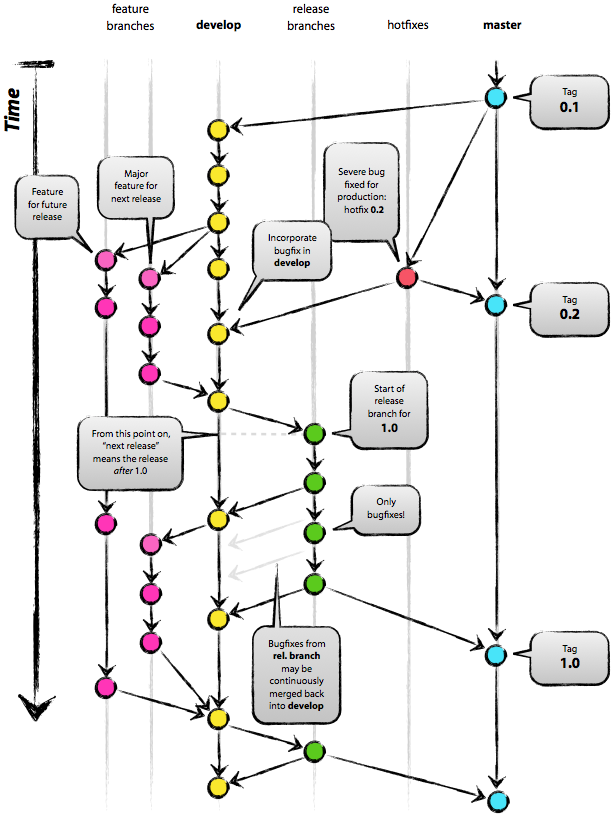
\includegraphics[height=170px, width=260px]{branch-model.png} 
    \caption{El esquema de branches que manejamos. \url{http://nvie.com/posts/a-successful-git-branching-model/}}
  \end{figure}
\end{frame}

\subsection{Tags}

\begin{frame}[fragile]{Tagging}
  \begin{block}{Listar}
    \begin{verbatim}
  $ git tag
    \end{verbatim}
  \end{block} 
  \pause
  \begin{block}{Crear un tag}
    \begin{verbatim}
  $ git tag -a v1.4 -m "creando el tag 1.4"
    \end{verbatim}
  \end{block}
  \pause
  \begin{block}{Eliminarlo}
    \begin{verbatim}
  $ git push origin :refs/tags/v1.4
    \end{verbatim}
  \end{block}
  \footnotetext{Para más información: \url{http://git-scm.com/book/en/Git-Basics-Tagging}}
\end{frame}


\section{Adicionales}

\subsection{Tips: Stash, Cherry, Cherry pick}

\begin{frame}{Stash}
  \begin{block}{Stash}
  ¿Qué pasa si estoy por la mitad de un cambio y necesito moverme de branch para ver otra cosa? Si intentamos
  hacer checkout, nos va a pedir que commiteemos los cambios ya que de otra manera los vamos a perder. Otra opción
  es el comando \textbf{stash}. \footnotemark \\
  Básicamente, la idea es que los cambios quedan almacenados y al hacer git status no los vemos. Una vez que volvamos
  a trabajar en ese branch, podemos recuperarlos con git stash apply.
  \end{block}
  
  \footnotetext{Para más información: \url{http://git-scm.com/book/en/Git-Tools-Stashing}}
\end{frame}

\begin{frame}{Cherry - Cherry Pick}
  \begin{block}{Cherry}
  En ciertas circunstancias podríamos llegar a necesitar aplicar cambios en ramas que divergieron. Es decir, si 
  las mergeara, traería otros cambios que yo no quiero. El comando cherry nos permite ver, dado un branch, qué cambios
  se hicieron desde que las dos ramas se separaron. \url{http://git-scm.com/docs/git-cherry}.
  \end{block}
  \pause
  \begin{block}{Cherry Pick}
  Cherry pick nos permite aplicar esos cambios de uno o más commits específicos a un branch. \url{http://git-scm.com/docs/git-cherry-pick}.
  \end{block}
\end{frame}

\subsection{Gitignore}

\begin{frame}{Gitignore}
  \begin{block}{.gitignore}
      Tenemos la posibilidad de decirle a git que ignore cierto patrón de archivos en el índice. Para ello basta crear un archivo con el nombre .gitignore
      y escribir adentro los nombres de archivos o carpetas que queremos ignorar. Si queremos que aplique a todo el repositorio, lo ponemos en la raíz.
      Si es más específico pueden agregarse múltiples en diferentes carpetas. Algo importante es nunca poner .gitignore adentro ya que el .gitignore en
      sí mismo debe ser commiteado para que afecte a todos los que utilizan el repositorio.
  \end{block}

\end{frame}

\subsection{Svn2Git}

\begin{frame}{Svn2Git}
  \begin{block}{}
      Svn2Git es una herramienta open-source que nos sirve para migrar un repositorio svn a git, sin perder el historial.
      Para descarga y documentación: \url{https://github.com/nirvdrum/svn2git/}
  \end{block}

\end{frame}

\subsection{Referencias}

\begin{frame}{Referencias}
 \begin{block}{Links útiles}
    \begin{itemize}
     \item Git official website, \url{http://git-scm.com/}
     \item Pro Git Book, \url{http://git-scm.com/book}
     \item Git Tutorial, \url{http://www.slideshare.net/eykanal/git-introductory-talk}
     \item Git guía rápida, \url{http://www.edy.es/dev/docs/git-guia-rapida/}
     \item Basic branching and merging, \url{http://git-scm.com/book/en/Git-Branching-Basic-Branching-and-Merging}
     \item A successful branch model, \url{http://nvie.com/posts/a-successful-git-branching-model/}
    \end{itemize}

 \end{block}
\end{frame}

\begin{frame}{Referencias (2)}
 \begin{block}{Links útiles}
    \begin{itemize}
          \item Some git tips, \url{http://mislav.uniqpath.com/2010/07/git-tips/}
     \item Revert commit by hash, \url{http://stackoverflow.com/questions/1895059/git-revert-to-a-commit-by-sha-hash}
     \item Revert bad merge, \url{https://condor-wiki.cs.wisc.edu/index.cgi/wiki?p=RevertingBadMerges}
    \end{itemize}

 \end{block}
\end{frame}


\end{document}